\documentclass{beamer}

\mode<presentation>{
\usetheme{Madrid}
%\usecolortheme{beaver}
}
\usepackage[utf8]{inputenc}
\usepackage{default}
\usepackage[portuguese]{babel}
\usepackage{pgfplots}
\pgfplotsset{/pgf/number format/use comma,compat=newest}
\usepackage{color}
\usepackage{amsmath,amsfonts,amssymb}
\usepackage{hyperref}
\usepackage{tikz}
% Para imagens
\usepackage{graphicx}
\usepackage{subcaption}
% Para imagens ao lado de texto
\usepackage{wrapfig}
%\usepackage{float} % necessário para manter as imagens no lugar certo
%Para a tabela
%\usepackage{tabu}
%\usepackage{tabularx}
%\usepackage{multirow}


\usebackgroundtemplate{%
\tikz\node[opacity=0.05] {
\includegraphics[height=\paperheight,width=\paperwidth]{logo_IME.png}};}


\title[Energia em IoT]{Aplicação de Internet das Coisas no Projeto Cisternas nas Escolas}
\author[Marcelo Schmitt]{Marcelo Schmitt}
\institute[IME-USP]{Universidade de São Paulo}
%\date{\today}
\date{}

\begin{document}

\begin{frame}
 \maketitle
\end{frame}

\begin{frame}
\frametitle{Sumário}
 \tableofcontents
\end{frame}

\section{O Projeto}
\begin{frame}
\frametitle{ONG Engenheiros Sem Fronteiras}
\begin{minipage}{\textwidth}

\begin{wrapfigure}{r}{0.5\textwidth}
	\vspace{-10pt}
	\begin{center}
		
\includegraphics[width=0.4\textwidth]{eng_sem_front.png}
	\end{center}
	%\caption{}
\end{wrapfigure}

A ONG Engenheiros Sem Fronteiras Brasil é uma organização sem fins lucrativos que acredita na utilização da engenharia como meio de transformação social.

\end{minipage}
\end{frame}

\begin{frame}
\frametitle{Projeto Cisternas nas Escolas}
\begin{minipage}{\textwidth}

	\begin{wrapfigure}{r}{0.5\textwidth}
		\begin{center}
			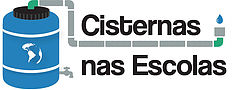
\includegraphics[width=0.35\textwidth]{logo.jpg}
		\end{center}
		%\caption{A gull}
		\vspace{+15pt}
	\end{wrapfigure}

	O Projeto Cisternas nas Escolas tem como objetivo construir sistemas de captação de água de chuva em escolas da rede pública de São Paulo e realizar atividades educacionais com base no projeto de engenharia para desenvolver habilidades de correlação e raciocínio lógico.\\
	
	Em 2017 foi implantado em duas escolas:
	\begin{itemize}
		\item EMEF Olavo Pezzotti 
		\item EMEI Alberto de Oliveira
	\end{itemize}

\end{minipage}
\end{frame}

\begin{frame}
\frametitle{Projeto Cisternas nas Escolas - Implatanção}
\begin{minipage}{\textwidth}

	\begin{figure}
		\vspace{+10pt}
		\centering
		\begin{subfigure}{0.3\textwidth}
			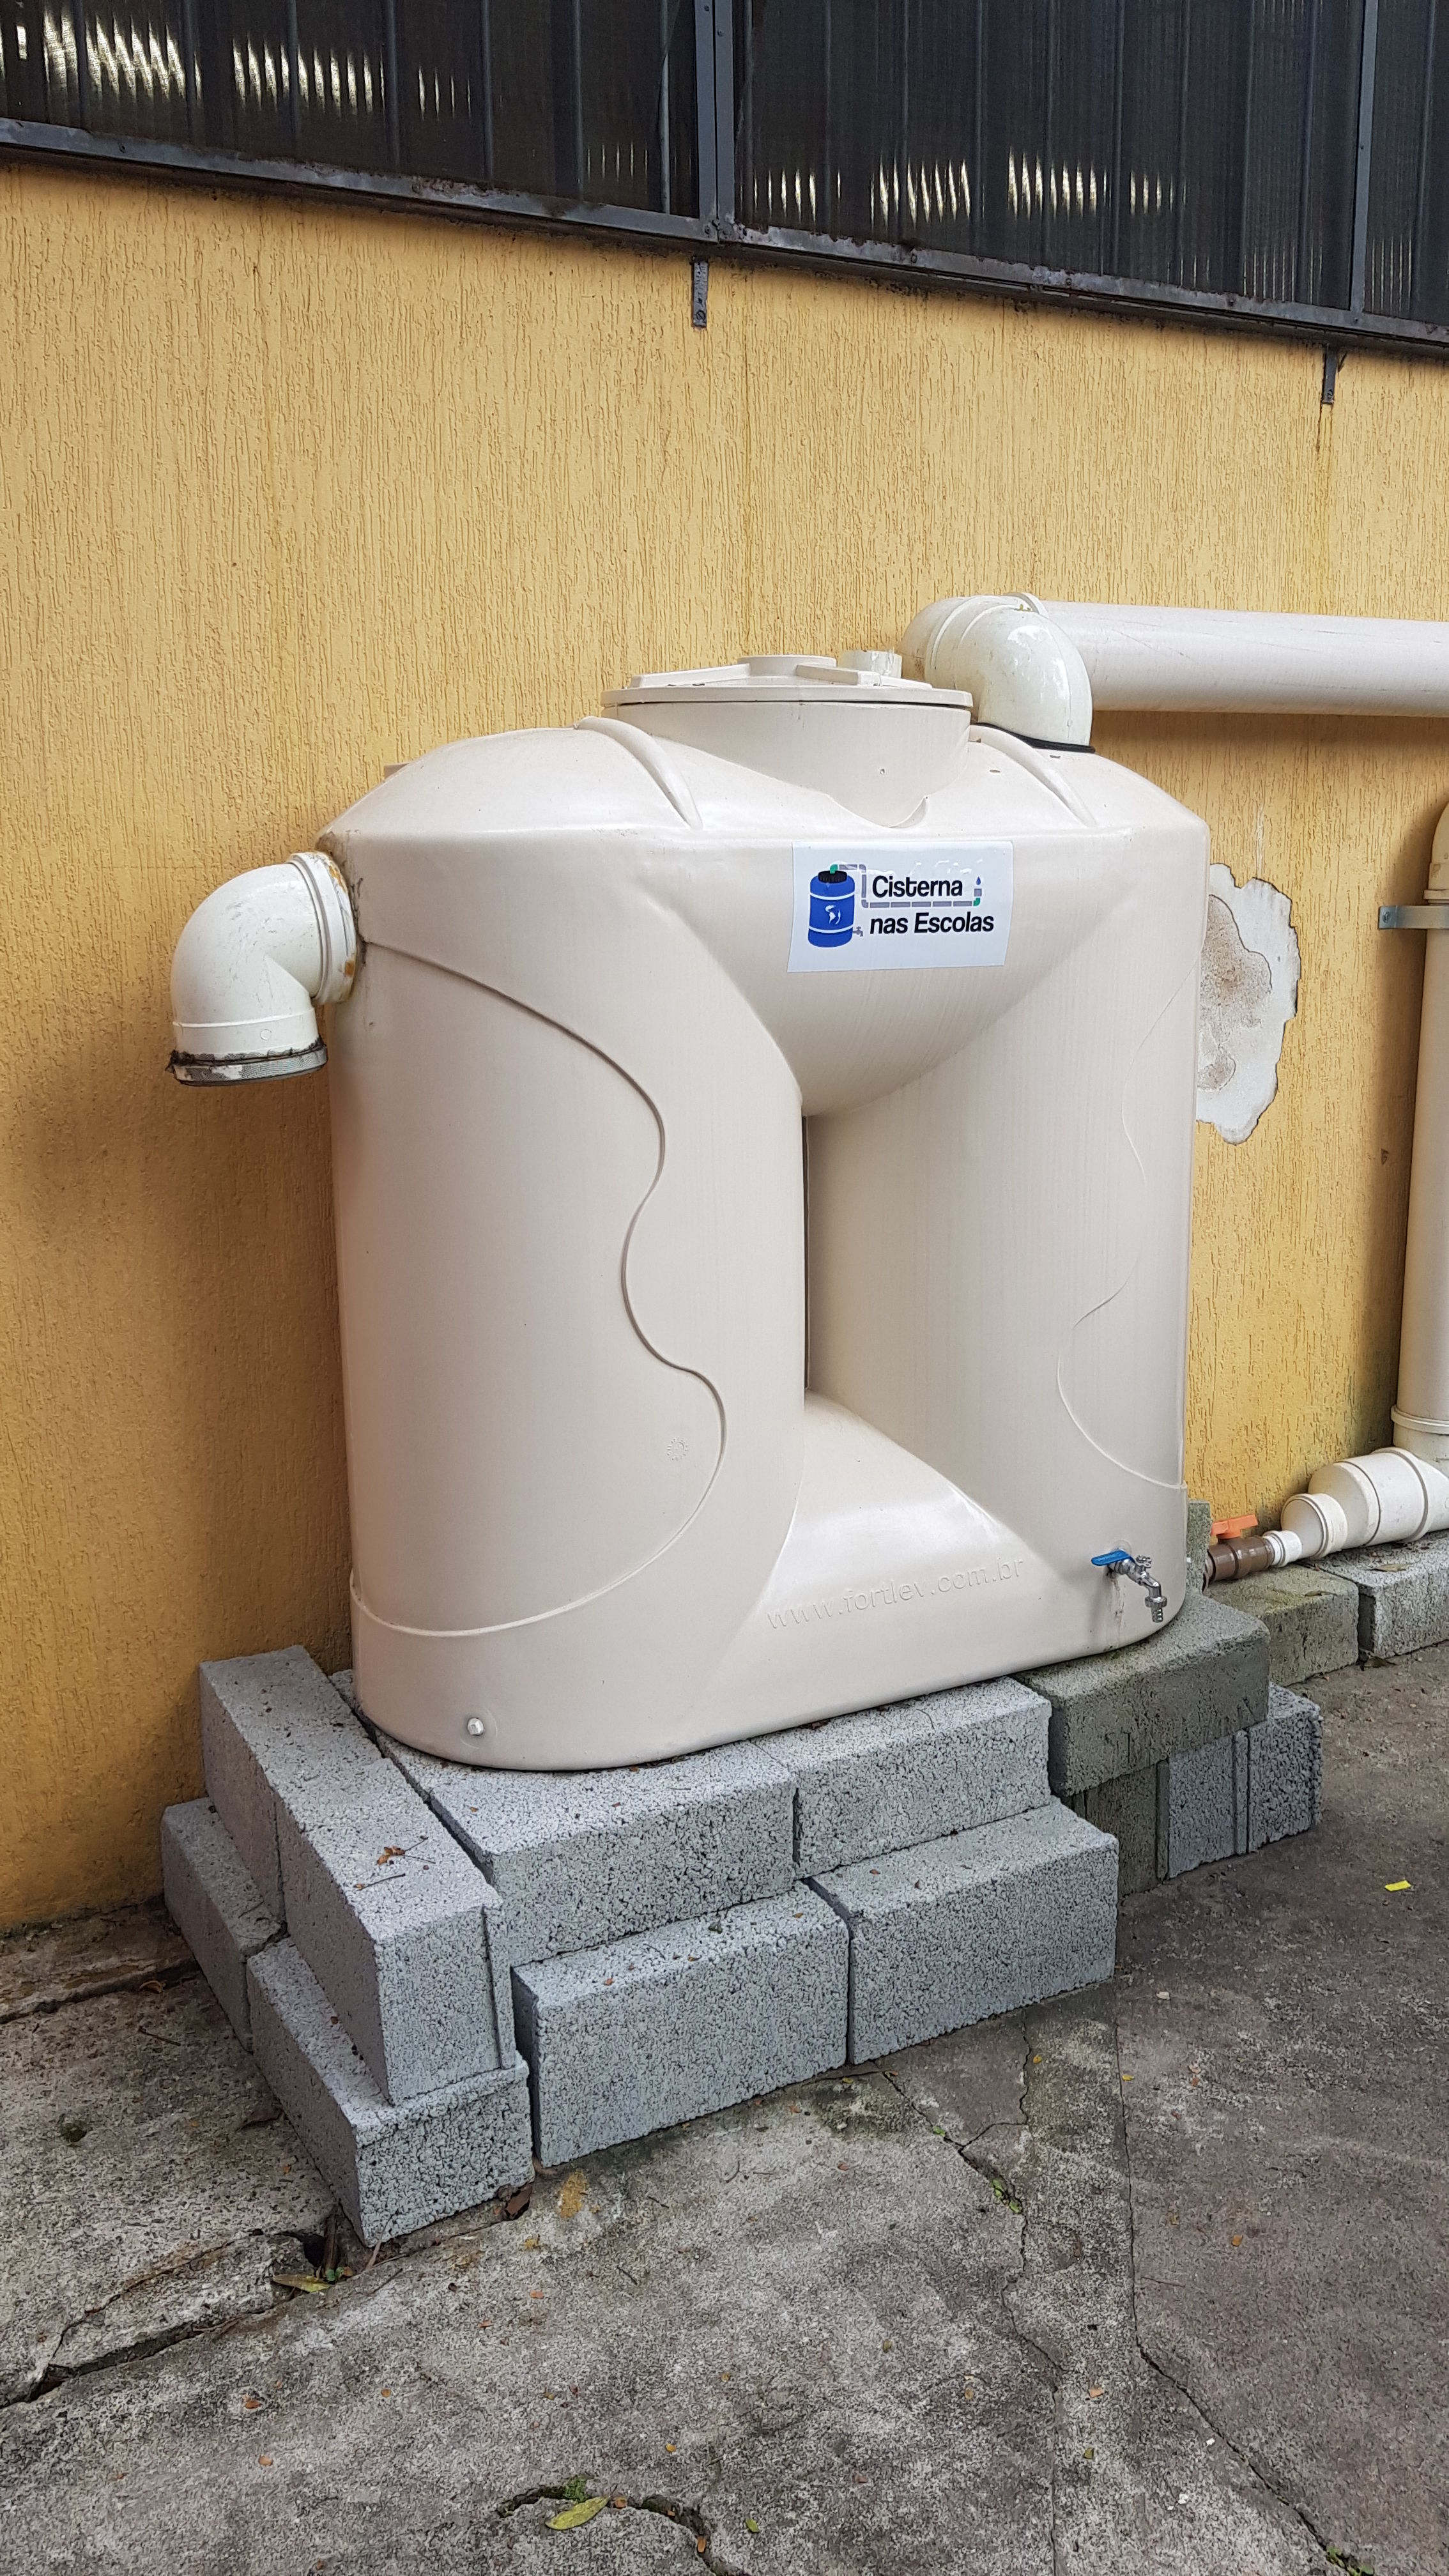
\includegraphics[width=\textwidth]{foto_cisterna2.jpg}
			%\caption{Sisterna instalada na EMEF Olavo Pezzotti}
			%\label{fig:arudinddfo_uno}
		\end{subfigure}
		\quad
		\begin{subfigure}{0.48\textwidth}
			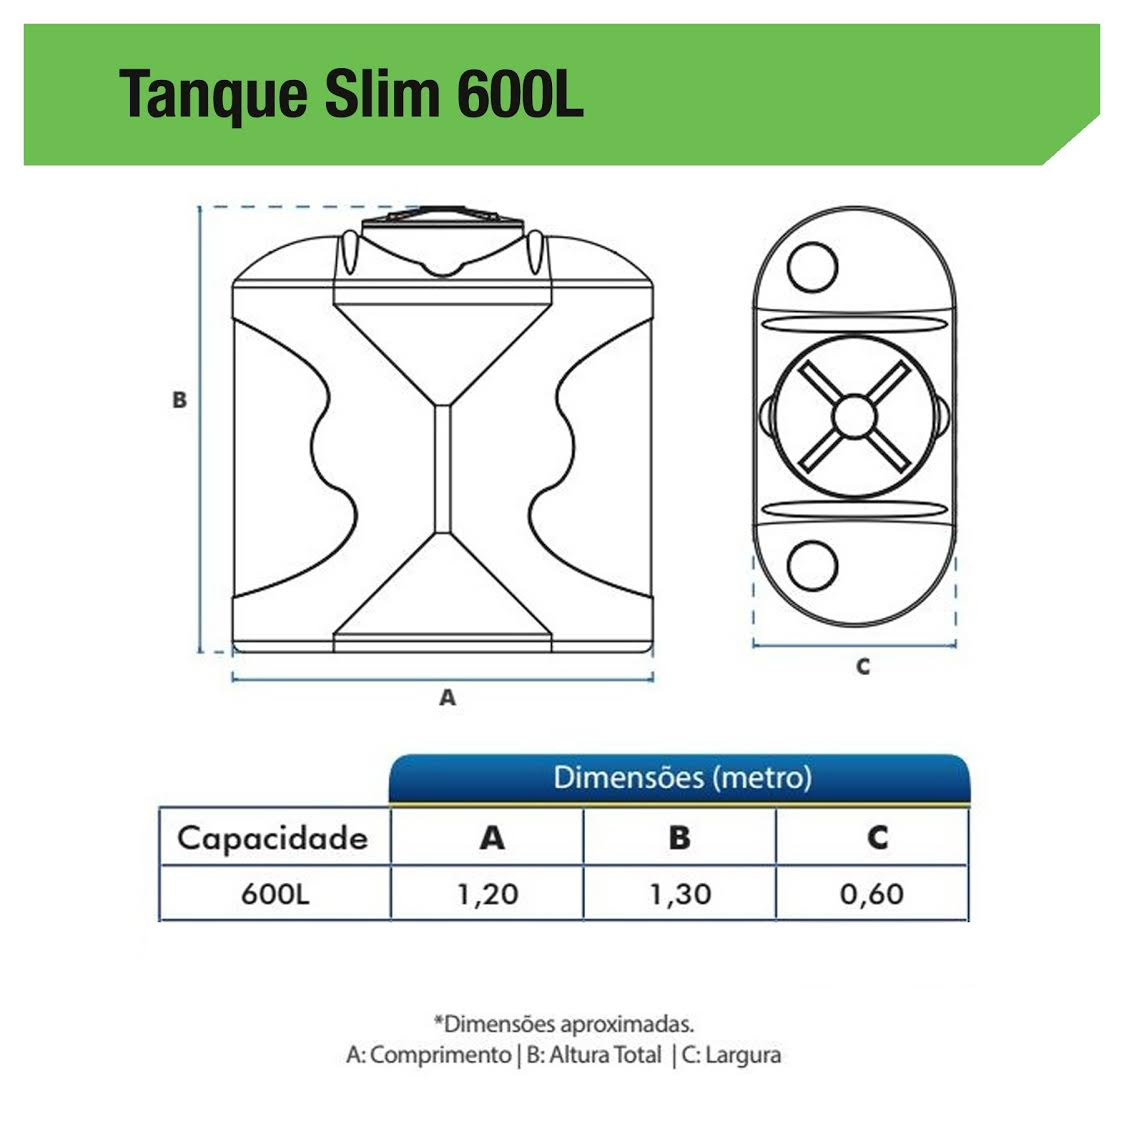
\includegraphics[width=\textwidth]{dimensoes_cisterna.jpg}
			%\caption{Modelo esquemático da cisterna}
			%\label{fig:node_mcudfd}
		\end{subfigure}
		\caption{Sisterna instalada na EMEF Olavo Pezzotti}
		\label{fig:plfdacddsfa_iot}
		\vspace{-10pt}
	\end{figure}

	%Em 2017, foram implementados 2 projetos técnico-educacionais de captação de água de chuva, um na Escola Municipal de Ensino Fundamental Olavo Pezzotti e outro na Escola Municipal de Ensino Infantil Alberto de Oliveira. A iniciativa foi contemplada pelo edital da Associação Amigos da Poli, que financiou ambos os projetos ao longo do ano.
	
\end{minipage}
\end{frame}

\section{Aplicação de IoT}

\begin{frame}
\frametitle{Internet das Coisas e o Projeto Cisternas nas Escolas}
\begin{minipage}{\textwidth}

	\begin{block}{}
		Para proporcionar uma melhor gestão da água captada pela cisterna, foi proposto fazer a mediação do volume de água contido nela. Essa informação deve ficar acessível para a diretoria da escola para que seja possível equilibrar de melhor forma o uso de água das chuvas e o uso de água da rede. Periodicamente funcionários do setor de limpeza devem adicionar cloro na cisterna. Como complemento ao sensor de nível de água será colocado um pequeno recipiente dentro da cisterna que despeje pastilhas de cloro periodicamente ou ao sinal de um comando em um interface web.
	\end{block}

	Público alvo interessado:
	\begin{itemize}
		\item Diretoria das escolas, para gerenciar o uso da água;
		\item Alunos, podem desenvolver interesse por ciência e engenharia a partir de projetos como esse;
		\item Governo do estado de São Paulo, pode monitorar o uso de recursos hídricos que as escolas fazem.
	\end{itemize}
\end{minipage}
\end{frame}

\begin{frame}
\frametitle{Arquitetura de IoT}
\begin{minipage}{\textwidth}
	%Apresentar como vocês pretendem tratar o fluxo de dados obtidos pelos sensores desde a coleta até chegar a uma informação e ação inteligente.
		
	\begin{figure}[!ht]
		\centering
		\vspace{-20pt}
		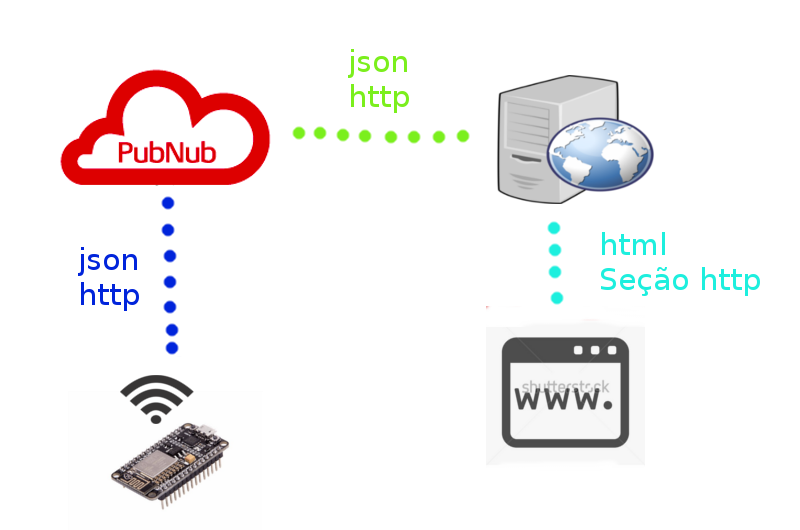
\includegraphics[width=0.8\textwidth]{arquitetura_projeto.png}
		\caption{Arquitetura da solução de IoT}
		\label{fig:ndfgodsdfsde_power_pisdfdns}
		%\vspace{-10pt}
	\end{figure}
	
\end{minipage}
\end{frame}

\section{Componentes da Solução de IoT}

\begin{frame}
\frametitle{Sensor}
\begin{minipage}{\textwidth}
		
		%Sensores: Quais sensores serão utilizados, onde eles poderão ser instalados, e a razão dessas escolhas.
		
		%Descrição técnica dos sensores: Apresentar os dados técnicos incluindo as características apresentadas no curso.
		
	\begin{wrapfigure}{r}{0.35\textwidth}
		\vspace{+20pt}
		\begin{center}
			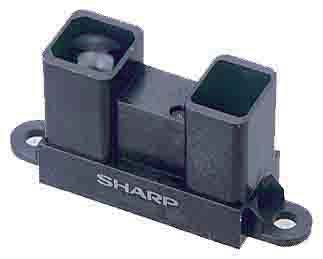
\includegraphics[width=0.3\textwidth]{sharp_sensor.jpg}
		\end{center}
		%\caption{Sensor Sharp}
	\end{wrapfigure}
	
	O Sharp GP2Y0A02YK0F é um sensor de distância composto por um IRED (diodo emissor de infravermelho) e uma unidade de porcessamento de sinal.

	Características:
	
	\begin{itemize}
		\item Intervalo de medição: 20 a 150cm
		\item Saída analógica
		\item Consumo de corrente: 33mA
		\item Voltagem de operação: 4.5 to 5.5 V
		\item Temperatura de opreação: -10 a +60 ºC
	\end{itemize}
		
\end{minipage}
\end{frame}

\begin{frame}
\frametitle{Uso do sensor Sharp}
\begin{minipage}{\textwidth}

	\begin{figure}[!ht]
		\vspace{-2pt}
		\centering
		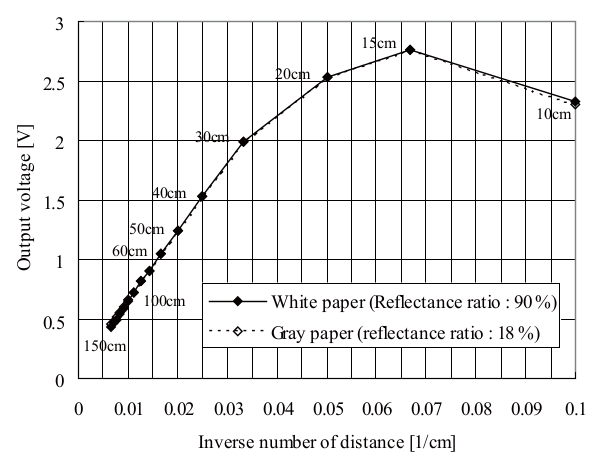
\includegraphics[width=0.75\textwidth]{grafico_calibracao_sensor.png}
		\vspace{-10pt}
		\caption{Gráfico utilizado para a calibração do sensor. Note que a voltagem de saída é aproximadamente linearmente proporcional ao inverso da distância até o objeto quando ele está entre 20 e 150cm de distância do sensor.}
		\label{fig:aligfgfmentacdffdao_usb}
	\end{figure}

\end{minipage}
\end{frame}

\begin{frame}
\frametitle{Placa de IoT}
\begin{minipage}{\textwidth}
		
	\begin{wrapfigure}{r}{0.3\textwidth}
		%\vspace{-20pt}
		\begin{center}
			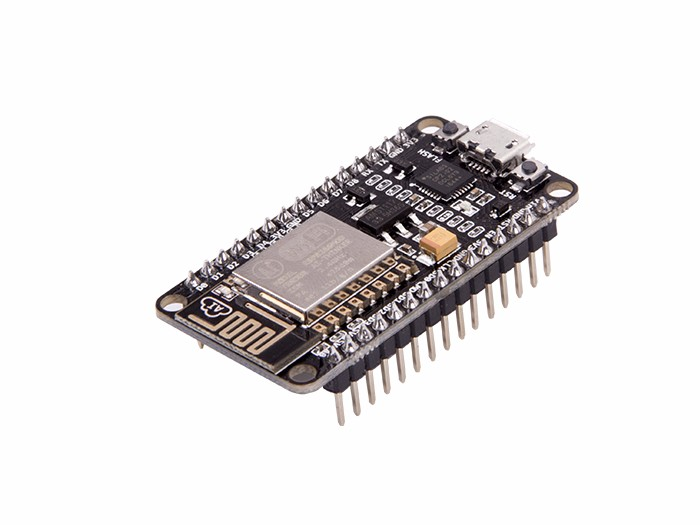
\includegraphics[width=0.3\textwidth]{NodeMCUAmica.jpg}
		\end{center}
		%\caption{A gull}
	\end{wrapfigure}

	O NodeMCU Amica é uma placa de prototipagem rápida que implementa funções de conexão à Internet por WiFi.
	
	Características:

	\begin{itemize}
		\item Voltagem de alimentação 3.3-20V 
		\item Consumo máximo de corrente: 1000mA%\cite{nodemcu_amica_datasheet}
		\item Protocolos WiFi: 802.11 b/g/n support
		\item Temperatura de operação: -40 a +125ºC
		\item Segurança: WPA/WPA2
		\item Protocolos de rede: IPv4, TCP/UDP/HTTP/FTP
	\end{itemize}

\end{minipage}
\end{frame}

\begin{frame}
\frametitle{Plataforma de Streaming}
\begin{minipage}{\textwidth}
	
	\begin{wrapfigure}{r}{0.3\textwidth}
		%\vspace{-20pt}
		\begin{center}
			
\includegraphics[width=0.3\textwidth]{pubnub.png}
		\end{center}
		%\caption{A gull}
	\end{wrapfigure}
	O PubNub oferece um serviço de streaming de dados no modelo publisher subscriber (publicadores e receptores de conteúdo).
	
	Características:
	
	\begin{itemize}
		\item API RESTfull
		\item Vários canais para publicar e receber mensagens
		\item Armazenamento persistente
		\item Resposta em tempo real
		\item Gratuito (considerando uma quantidade moderada de mensagens)
	\end{itemize}
	
\end{minipage}
\end{frame}

\begin{frame}
\frametitle{Servidor Web}
\begin{minipage}{\textwidth}

	\begin{wrapfigure}{r}{0.3\textwidth}
		%\vspace{-20pt}
		\begin{center}
				
\includegraphics[width=0.3\textwidth]{web-server-pa-django.png}
		\end{center}
		%\caption{A gull}
	\end{wrapfigure}
	
	
	
	Django hospedado no PythonAnywhere. \\
	Django é um framework web de configuração e desenvolvimento rápido enquanto que PythonAnywhere é um ambiente de desenvolvimento integrado e serviço de hospedagem web.
	
	Característica:
	%O Django é um framework web de configuração e desenvolvimento rápido que incentiva um design de aplicação limpo e pragmático.
	
	%Django makes it easier to build better Web apps more quickly and with less code
	%Django is a high-level Python Web framework that encourages rapid development and clean, pragmatic design
	
	%Start hosting quickly
	%Just write your application. No need to configure or maintain a web server — everything is set up and ready to go.
	%PythonAnywhere é um ambiente de desenvolvimento integrado e serviço de hospedagem web baseado na linguagem de programação Python.
	\begin{itemize}
		\item Configuração rápida e fácil
		\item Templates prontos para controle de acesso a páginas html
		\item Gratuito (com várias limitações)
	\end{itemize}
		
\end{minipage}
\end{frame}

\begin{frame}
\frametitle{Atuador}
\begin{minipage}{\textwidth}
	
	%Sensores: Quais sensores serão utilizados, onde eles poderão ser instalados, e a razão dessas escolhas.
	
	%Descrição técnica dos sensores: Apresentar os dados técnicos incluindo as características apresentadas no curso.
	
	
	\begin{wrapfigure}{r}{0.3\textwidth}
		%\vspace{-20pt}
		\begin{center}
			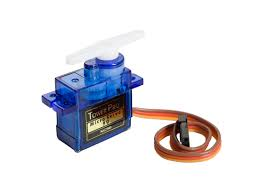
\includegraphics[width=0.3\textwidth]{servo.jpeg}
		\end{center}
		%\caption{A gull}
	\end{wrapfigure}
	
	O motor servo é pequeno e pode ser utilizado para abrir uma portilhola por onde seriam despejadas pastilhas de cloro na cisterna.
	
	\begin{itemize}
		\item Voltagem de operação: 4.8 a 6V
		\item Velocidade: 0,12 seg/60Graus (4,8V) sem carga
		\item Ângulo de rotação: 180 graus
		\item Temperatura de Operação: -30 a +60ºC
	\end{itemize}
	
\end{minipage}
\end{frame}

\begin{frame}
\frametitle{Exibição e Análise de Dados}
\begin{minipage}{\textwidth}
	
	A partir dos dados de coletados pode-se gerar gráficos de utilização e estimar o nível de água em um dado horário do dia.
	
	\begin{figure}[H]
		\centering
		%\vspace{-20pt}
		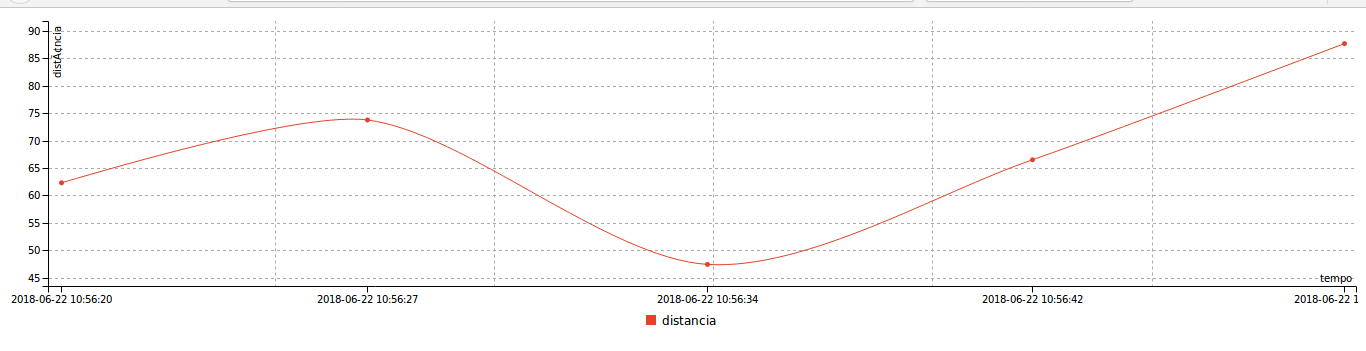
\includegraphics[width=0.9\textwidth]{grafico_distancia.png}
		\caption{Gráfico de nível de água na cisterna}
		\label{fig:nfgfdfgodsdfsde_power_pisdfdns}
		%\vspace{-10pt}
	\end{figure}
	
\end{minipage}
\end{frame}

\section{Dificuldades}

\begin{frame}
\frametitle{Algumas Dificuldades Encontradas}
\begin{minipage}{\textwidth}
	
	
	\begin{itemize}
		\item Encontrar um sensor apropriado
		\item Selecionar uma placa de IoT que melhor se adapta-se às necessidades do projeto
		\item Escolher um serviço de stream de dados com uma API que facilitasse enviar e receber mensagens em ambas as pontas da comunicação
		
	\end{itemize}

\end{minipage}
\end{frame}

\begin{frame}
\frametitle{Conclusão}
\begin{minipage}{\textwidth}
	Imbutir funcionalidades de IoT no Projeto Cisternas nas Escolas resultou em um trabalho bem amplo pois várias ferramentes de computação podem ser aplicadas na sua melhoria. Ao mesmo tempo também pode se tornar difícil selecionar dentre as várias ferramentas com funcionalidades semelhantes disponíveis para o uso.
\end{minipage}
\end{frame}

\section{Referências}
\begin{frame}
	\frametitle{Referências}
	\begin{thebibliography}{5}
		%\bibitem{beamer} \emph{Tantau T., Wright J. and Mileti\'{c} V. The BEAMER class - User Guide for version 3.36, March 2015}.
		%\bibitem{beamer2} \emph{Mertz A. and Slough W. Beamer by Example. The Prac\TeX~ Journal, n. 4, 2005.}
		%\bibitem{beamer1} \emph{Mohammad, et al.Machine Learning for Internet of Things Data Analysis - A Survey. Disponível em: \url{Suveri https://arxiv.org/pdf/1802.06305.pdf}}
		%\bibitem{beamer2} \emph{A. Mostafa, Yaser. - Learning From Data. Disponível em: \url{http://www.youtube.com/watch?v=FIbVs5GbBlQ&hd=1}}
		
		%\bibitem{beamer4} \emph{\url{https://en.wikipedia.org/wiki/Naive\_Bayes\_classifier}}
		
		\bibitem{esfsp}\href{http://www.esfsaopaulo.org/}{Engenheiros Sem Fronteira - Núcleo São Paulo}
		
		\bibitem{projeto_cisternas_nas_escolas}\href{http://www.esfsaopaulo.org/projetos}{Projeto Cisternas nas Escolas}
		
		\bibitem{datasheet_sharp}\href{https://www.pololu.com/file/0J156/gp2y0a02yk_e.pdf}{Sharp GP2Y0A02YK0F - Datasheet}
		
		\bibitem{nodemcu_amica_datasheet}\href{https://github.com/nodemcu/nodemcu-devkit-v1.0/blob/master/NODEMCU_DEVKIT_V1.0.PDF}{NodeMCU Amica - Datasheet}
		
		\bibitem{pubnub_home}\href{https://www.pubnub.com/}{PubNub}
		
		\bibitem{django_home}\href{https://www.djangoproject.com/}{Framework django}
		
		\bibitem{pa_home}\href{https://www.pythonanywhere.com/}{Python Anywhere}
		
		\bibitem{servo_spec}\href{https://www.filipeflop.com/produto/micro-servo-9g-sg90-towerpro/}{Especificações do micro-servo-9g-sg90-towerpro}
				
		\bibitem{sensor_capacitivo}\href{http://www.instructables.com/id/Capacitive-Fluid-Level-Sensor/}{Sensor de nível de água capacitivo}
		
		
		%\bibitem{espressif}\href{https://www.espressif.com/sites/default/files/documentation/0a-esp8266ex_datasheet_en.pdf}{ESP8266EX - Datasheet}
		
		
	\end{thebibliography}
	
\end{frame}


\end{document}
